\documentclass[11pt]{article}
\newcommand{\ArticleShortTitle}{Upfront BVC для программирования}
\newcommand{\ArticlePDFTitle}{Предварительное многоролевое планирование для программирования и vibe coding}
\usepackage[a4paper,top=22mm,bottom=22mm,left=22mm,right=22mm,headheight=22pt]{geometry}
\usepackage{fontspec}
\defaultfontfeatures{Ligatures=TeX,Scale=MatchLowercase}
\setmainfont{times.ttf}[
  Path=C:/Windows/Fonts/,
  BoldFont=timesbd.ttf,
  ItalicFont=timesi.ttf,
  BoldItalicFont=timesbi.ttf
]
\setsansfont{arial.ttf}[
  Path=C:/Windows/Fonts/,
  BoldFont=arialbd.ttf,
  ItalicFont=ariali.ttf,
  BoldItalicFont=arialbi.ttf
]
\setmonofont{consola.ttf}[
  Path=C:/Windows/Fonts/,
  BoldFont=consolab.ttf,
  ItalicFont=consolai.ttf,
  BoldItalicFont=consolaz.ttf,
  Scale=0.82
]
\usepackage[main=russian,english]{babel}
\usepackage{microtype}

\usepackage{amsmath,amssymb,mathtools}
\usepackage{booktabs,tabularx,array,longtable,multirow}
\usepackage{graphicx}
\graphicspath{{figures/}}
\usepackage{float}
\usepackage[section]{placeins}
\usepackage{caption}
\usepackage{subcaption}
\usepackage{enumitem}
\usepackage{siunitx}
\sisetup{
  output-decimal-marker={,},
  group-separator={\,},
  group-minimum-digits=4,
  detect-all
}
\usepackage{xcolor}
\definecolor{Ink}{HTML}{0F172A}
\definecolor{Muted}{HTML}{475569}
\definecolor{Rule}{HTML}{CBD5E1}
\definecolor{BVC}{HTML}{7C3AED}
\definecolor{Cyan}{HTML}{0EA5E9}
\definecolor{Teal}{HTML}{14B8A6}
\definecolor{Amber}{HTML}{F59E0B}
\definecolor{Soft}{HTML}{F8FAFC}
\usepackage[most]{tcolorbox}
\newtcolorbox{resultbox}[1][]{
  enhanced,
  breakable,
  colback=Soft,
  colframe=BVC,
  boxrule=0.8pt,
  arc=1.5mm,
  left=3mm,right=3mm,top=2mm,bottom=2mm,
  title={#1},
  fonttitle=\bfseries\sffamily,
  coltitle=Ink
}
\newtcolorbox{methodbox}[1][]{
  enhanced,
  breakable,
  colback=white,
  colframe=Rule,
  boxrule=0.6pt,
  arc=1.5mm,
  left=3mm,right=3mm,top=2mm,bottom=2mm,
  title={#1},
  fonttitle=\bfseries\sffamily,
  coltitle=Ink
}

\usepackage{tikz}
\usetikzlibrary{arrows.meta,positioning,shapes.geometric,calc,fit}
\tikzset{
  stage/.style={draw=Rule,rounded corners=2mm,fill=Soft,minimum height=11mm,
    text width=28mm,align=center,font=\small\sffamily},
  gate/.style={diamond,draw=BVC,fill=BVC!7,aspect=1.8,align=center,
    inner sep=1.2mm,font=\small\sffamily},
  flow/.style={-{Latex[length=2.2mm]},thick,draw=Muted},
  note/.style={font=\scriptsize\sffamily,text=Muted,align=center}
}

\usepackage{titlesec}
\titleformat{\section}{\Large\bfseries\sffamily\color{Ink}}{\thesection.}{0.55em}{}
\titleformat{\subsection}{\large\bfseries\sffamily\color{Ink}}{\thesubsection.}{0.55em}{}
\titleformat{\subsubsection}{\normalsize\bfseries\sffamily\color{Ink}}{\thesubsubsection.}{0.55em}{}
\titlespacing*{\section}{0pt}{2.2ex plus .5ex minus .2ex}{1.0ex}
\titlespacing*{\subsection}{0pt}{1.8ex plus .4ex minus .2ex}{0.8ex}

\usepackage{fancyhdr}
\pagestyle{fancy}
\fancyhf{}
\fancyhead[L]{\small\sffamily\color{Muted}\ArticleShortTitle}
\fancyhead[R]{\small\sffamily\color{Muted}Xynapse / BVC}
\fancyfoot[C]{\small\sffamily\color{Muted}\thepage}
\renewcommand{\headrulewidth}{0.4pt}
\renewcommand{\headrule}{\hbox to\headwidth{\color{Rule}\leaders\hrule height \headrulewidth\hfill}}

\usepackage{csquotes}
\usepackage[
  backend=biber,
  style=numeric-comp,
  sorting=nyt,
  maxbibnames=8,
  giveninits=true,
  doi=true,
  url=true,
  isbn=false
]{biblatex}
\addbibresource{references.bib}
\AtBeginBibliography{\footnotesize\sloppy\hbadness=10000\relax}

\usepackage{hyperref}
\hypersetup{
  colorlinks=true,
  linkcolor=BVC,
  citecolor=BVC,
  urlcolor=Cyan,
  pdftitle={\ArticlePDFTitle},
  pdfauthor={Халилов Джабраиль Эльнурович},
  pdfsubject={Экспериментальная оценка BVC},
  pdfkeywords={BVC, SWE-bench Verified, LLM, программирование, Xynapse}
}
\usepackage[nameinlink,noabbrev]{cleveref}

\captionsetup{
  font=small,
  labelfont={bf,sf,color=Ink},
  textfont={color=Muted},
  justification=centering,
  singlelinecheck=false,
  skip=5pt
}
\setlist[itemize]{leftmargin=1.5em,itemsep=0.25em,topsep=0.35em}
\setlist[enumerate]{leftmargin=1.6em,itemsep=0.25em,topsep=0.35em}
\renewcommand{\arraystretch}{1.15}
\setlength{\tabcolsep}{5pt}
\setlength{\parindent}{1.15em}
\setlength{\parskip}{0.18em}
\setlength{\emergencystretch}{4em}
\tolerance=1200

\newcommand{\BVCname}{Bounded Verification Council (BVC)}
\newcommand{\pp}{п.\,п.}
\newcommand{\dataset}{SWE-bench Verified}
\newcommand{\code}[1]{\texttt{#1}}
\newcommand{\sourcehash}[1]{\texttt{\footnotesize #1}}

% Auto-generated by generate_analysis_assets.py. Do not edit by hand.
\newcommand{\NTasks}{60}
\newcommand{\NRepos}{11}
\newcommand{\NPrimaryRuns}{240}
\newcommand{\NRepeatRuns}{90}
\newcommand{\NVibeRuns}{45}
\newcommand{\NAllRuns}{375}
\newcommand{\DirectResolved}{4}
\newcommand{\SingleResolved}{7}
\newcommand{\BVCResolved}{5}
\newcommand{\FixedResolved}{6}
\newcommand{\DirectRate}{6.7}
\newcommand{\SingleRate}{11.7}
\newcommand{\BVCRate}{8.3}
\newcommand{\FixedRate}{10.0}
\newcommand{\DirectWilsonLow}{2.6}
\newcommand{\DirectWilsonHigh}{15.9}
\newcommand{\SingleWilsonLow}{5.8}
\newcommand{\SingleWilsonHigh}{22.2}
\newcommand{\BVCWilsonLow}{3.6}
\newcommand{\BVCWilsonHigh}{18.1}
\newcommand{\FixedWilsonLow}{4.7}
\newcommand{\FixedWilsonHigh}{20.1}
\newcommand{\BVCCalls}{472}
\newcommand{\FixedCalls}{600}
\newcommand{\DirectCalls}{60}
\newcommand{\SingleCalls}{120}
\newcommand{\BVCTokens}{14282809}
\newcommand{\FixedTokens}{18365172}
\newcommand{\DirectTokens}{1867093}
\newcommand{\SingleTokens}{3585838}
\newcommand{\BVCCost}{1838.46}
\newcommand{\FixedCost}{2402.61}
\newcommand{\DirectCost}{312.44}
\newcommand{\SingleCost}{522.84}
\newcommand{\BVCCostTask}{30.64}
\newcommand{\FixedCostTask}{40.04}
\newcommand{\DirectCostTask}{5.21}
\newcommand{\SingleCostTask}{8.71}
\newcommand{\BVCCostResolved}{367.69}
\newcommand{\FixedCostResolved}{400.44}
\newcommand{\DirectCostResolved}{78.11}
\newcommand{\SingleCostResolved}{74.69}
\newcommand{\CallsSaved}{128}
\newcommand{\CallsSavedPct}{21.3}
\newcommand{\TokensSaved}{4082363}
\newcommand{\TokensSavedPct}{22.2}
\newcommand{\CostSaved}{564.15}
\newcommand{\CostSavedPct}{23.5}
\newcommand{\CostResolvedSavedPct}{8.2}
\newcommand{\TokensSavedTask}{68039}
\newcommand{\CostSavedTask}{9.40}
\newcommand{\CallsSavedTaskMean}{2.13}
\newcommand{\CallsSavedTaskMeanLow}{1.60}
\newcommand{\CallsSavedTaskMeanHigh}{2.67}
\newcommand{\CallsSavedTaskMedian}{4}
\newcommand{\TokensSavedTaskMeanLow}{51980}
\newcommand{\TokensSavedTaskMeanHigh}{83480}
\newcommand{\TokensSavedTaskMedian}{111910}
\newcommand{\CostSavedTaskMeanLow}{6.75}
\newcommand{\CostSavedTaskMeanHigh}{12.05}
\newcommand{\CostSavedTaskMedian}{7.92}
\newcommand{\TokensOverrunTasks}{11}
\newcommand{\TokensOverrunMax}{13971}
\newcommand{\CostOverrunTasks}{10}
\newcommand{\CostOverrunMax}{12.84}
\newcommand{\BVCShort}{32}
\newcommand{\BVCExtended}{28}
\newcommand{\BVCShortResolved}{5}
\newcommand{\BVCExtendedResolved}{0}
\newcommand{\BVCShortTokensMean}{179160}
\newcommand{\BVCExtendedTokensMean}{305345}
\newcommand{\BVCShortCostMean}{22.78}
\newcommand{\BVCExtendedCostMean}{39.62}
\newcommand{\FixedShortResolved}{5}
\newcommand{\FixedExtendedResolved}{1}
\newcommand{\GateUndefinedVote}{7}
\newcommand{\GateFourValidAxes}{35}
\newcommand{\GateThreeValidAxes}{18}
\newcommand{\GateZeroValidAxes}{7}
\newcommand{\GateMetricCorrelation}{0.412}
\newcommand{\AllTokens}{54533372}
\newcommand{\AllCost}{7266.84}
\newcommand{\CostCap}{11800}



\title{\vspace{-1.2em}\textbf{\sffamily Предварительное многоролевое планирование\\
для программирования и vibe coding}}
\author{Халилов Джабраиль Эльнурович\\
\small Национальный исследовательский университет «Высшая школа экономики»\\
\small Исследовательский проект Xynapse / BVC\\
\small \href{https://github.com/jabrailkhalil/xynapse}{\nolinkurl{github.com/jabrailkhalil/xynapse}}}
\date{2026}

\begin{document}
\maketitle

\begin{abstract}
В интерактивном программировании пользователь часто понимает необходимость
дополнительной проверки до изменения кода: например, когда план составлен
несколькими агентами, дефект затрагивает несколько компонентов или цена
ошибочного первого решения высока. В статье исследуется upfront-сценарий
Bounded Verification Council (BVC), который человек явно включает до первой
правки. Его практическая сила состоит в понятном контракте: четыре роли
независимо анализируют причину, стратегию, зависимости и тесты;
формализованный gate либо немедленно синтезирует план, либо добавляет один
ограниченный раунд критики. На 60 реальных задачах \dataset{} BVC решил
5 задач против 7 у одного предварительного плана: первичная разность
\(-3{,}3\) процентного пункта, 95\% интервал
\([-10{,}0;+3{,}3]\), \(p=0{,}625\); преимущество и заранее заданная
неухудшаемость с margin \(-5\) \pp{} не установлены. Во вторичном сравнении
BVC решил 5 задач против 4 у прямой генерации patch: описательная разность
\(+1{,}7\) процентного пункта, 95\% стратифицированный bootstrap-интервал
\([0{,}0;+5{,}0]\), точный и Holm-adjusted \(p=1{,}0\). Это положительный
сигнал, но не
статистическое доказательство преимущества качества. В контролируемой
15-задачной разговорной серии BVC решил 1 задачу против 0 в формальной
постановке и сохранил одинаковый outcome на 14/15 задачах. Одновременно gate
завершил 32/60 задач коротким маршрутом и сократил токены на 22,2\%
относительно полного совета. Результаты показывают, как предложенный в
дипломе интерфейс Xynapse можно превратить в полезный и прозрачный режим
\enquote{сначала проверить план, затем писать код} с измеримым бюджетом и
честной границей статистических утверждений.
\end{abstract}

\noindent\textbf{Ключевые слова:} vibe coding, AI-ассистент, предварительное
планирование, многоагентный анализ, исправление дефектов, Xynapse, BVC,
\dataset{}.

\section{Введение}

Разговорное программирование снижает стоимость формулировки задачи: человек
может описать желаемое поведение обычным языком и сразу перейти к генерации
изменений. Слабое место такого взаимодействия проявляется до первой правки.
Если исходная локализация дефекта неверна, последующий инструментальный цикл
может уверенно редактировать неподходящий файл, расширять поверхность patch и
исправлять симптомы вместо причины.

В настоящей работе термин \emph{vibe coding} операционализирован узко: это
одна созданная моделью разговорная переформулировка исходного требования при
неизменных кодовом контексте, модели, лимитах и evaluator, без последующего
диалога. Интерактивное программирование с уточнениями пользователя,
инструментами и несколькими циклами правки здесь не исследуется.

Практический ответ пользователя нередко звучит так: \enquote{сначала составь
план с агентами} или \enquote{перед исправлением ошибки проверь решение с
нескольких сторон}. Это не требование бесконечного автономного роя. Скорее,
пользователь хочет короткий этап принятия инженерного решения, отделённый от
редактирования кода.

В дипломе автора Xynapse описан как интеллектуальная среда разработки с
интегрированным AI-ассистентом, а BVC --- как механизм многоролевой проверки
до действия \cite{khalilov2026}. Настоящая работа проверяет этот сценарий на
реальных программных задачах. Центральное свойство называется
\emph{upfront activation}: алгоритм включается человеком до первой правки,
формирует единый план, а уже затем передаёт его patch-генератору. Актуальная
реализация Xynapse опубликована в репозитории проекта \cite{xynapse2026}; этим
самым ссылка на программный код отделяется от ссылки на описание архитектуры в
дипломе.

Исследование не сводится к сравнению красивых планов. Итоговый patch
оценивается официальными тестами \dataset{} \cite{jimenez2024swebench};
одни и те же задачи попарно проходят direct, один план и многоролевые режимы.
Дополнительная серия проверяет контролируемую разговорную формулировку.

\begin{resultbox}[Что проверено]
\begin{itemize}
  \item момент включения: BVC запускается до первой правки;
  \item реальный outcome: применимость patch и прохождение тестов;
  \item первичный contrast с одним планом и вторичный contrast с direct;
  \item чувствительность к одному разговорному paraphrase;
  \item повторяемость бинарного результата при temperature \(=0\);
  \item адаптивный бюджет 6 или 10 вызовов.
\end{itemize}
\end{resultbox}

\begin{resultbox}[Почему upfront BVC полезен пользователю]
\begin{itemize}
  \item алгоритм включается осознанно до первой правки, когда цена неверного
        направления ещё не превратилась в цепочку изменений;
  \item на выходе пользователь получает один проверяемый план с причиной,
        стратегией, зависимостями и тестами, а не набор несвязанных мнений;
  \item решение об углублении анализа принимает прозрачный gate, а не
        неограниченный агентный диалог;
  \item бюджет ограничен 6--10 вызовами и может быть показан в интерфейсе
        вместе с фактическими токенами и стоимостью;
  \item разговорная формулировка проходит через тот же строгий контракт
        анализа, что удобно для vibe-coding-сценария.
\end{itemize}
BVC тем самым добавляет перед генерацией кода компактный слой инженерного
решения: пользователь сохраняет контроль, а система делает основания плана
видимыми.
\end{resultbox}

\section{Upfront BVC как рабочий контракт}

\subsection{Когда пользователь включает алгоритм}

Upfront BVC уместен не для каждой автодополняемой строки. Он предназначен
для момента, когда пользователь ещё не разрешил менять код и хочет повысить
качество первого инженерного решения. Типовые входы:
\begin{itemize}
  \item необходимо исправить дефект с неочевидной причиной;
  \item предполагается изменение нескольких модулей или API-контракта;
  \item пользователь уже запросил план у нескольких агентов и хочет
        синтезировать их позиции;
  \item нужно заранее сформулировать тесты и регрессионные инварианты;
  \item разговорная постановка неоднозначна, но фактическое требование можно
        проверить по репозиторию.
\end{itemize}

Активация является явной. Это сохраняет контроль пользователя над ценой:
режим direct остаётся доступным для дешёвых и очевидных правок, а BVC
выбирается там, где ошибка первоначального плана потенциально дороже
нескольких дополнительных вызовов.

\begin{figure}[H]
\centering
\resizebox{0.98\textwidth}{!}{%
\begin{tikzpicture}[node distance=7mm and 8mm]
  \node[stage, text width=27mm] (request) {Разговорная или\\формальная задача};
  \node[stage, right=of request, text width=27mm] (activate) {Явное решение\\«включить BVC»};
  \node[stage, right=of activate, text width=30mm] (roles) {Architect\\Developer\\Reviewer\\Tester};
  \node[gate, below=10mm of roles] (gate) {Проверка\\расхождения};
  \node[stage, below=10mm of gate, text width=27mm] (critique) {Один раунд\\критики};
  \node[stage, right=12mm of gate, text width=27mm] (plan) {Единый\\проверяемый план};
  \node[stage, right=of plan, text width=27mm] (tools) {Patch\\и тесты};
  \draw[flow] (request) -- (activate);
  \draw[flow] (activate) -- (roles);
  \draw[flow] (roles) -- (gate);
  \draw[flow] (gate) -- node[note,left]{нужно} (critique);
  \draw[flow] (critique.east) -| (plan.south);
  \draw[flow] (gate) -- node[note,above]{достаточно} (plan);
  \draw[flow] (plan) -- (tools);
\end{tikzpicture}
}
\caption{Контракт upfront BVC: анализ отделён от редактирования кода.}
\label{fig:workflow}
\end{figure}

\subsection{Разделение ответственности}

Четыре роли не голосуют за свободный текст целиком. Они формируют
структурированные решения:
\begin{enumerate}
  \item \textbf{Architect}: локализация причины, границы и зависимости;
  \item \textbf{Developer}: конкретная стратегия изменения;
  \item \textbf{Reviewer}: совместимость, инварианты и нежелательные эффекты;
  \item \textbf{Tester}: наблюдаемое поведение и достаточные проверки.
\end{enumerate}
После независимого раунда gate измеряет расхождение \(D_{\mathrm{vote}}\) и
неполноту \(D_{\mathrm{cov}}\). Если требуется критика, каждая роль видит
структурированные позиции остальных и уточняет своё решение. Синтезатор
выдаёт один план, а patch-генератор получает уже согласованную спецификацию.

\subsection{Исполняемая последовательность одной сессии}

Фраза \enquote{включить алгоритм заранее} в эксперименте означает конкретный
порядок, а не общий совет писать более длинный prompt:
\begin{enumerate}
  \item пользователь фиксирует issue либо уже составленный набором агентов
        черновой план и включает BVC до первой правки;
  \item система прикрепляет одинаковый retrieval-контекст репозитория и
        запускает четыре независимых role-вызова;
  \item JSON каждого ответа валидируется по четырём обязательным осям;
        отсутствующие или некорректные поля не угадываются, а входят в
        \(D_{\mathrm{cov}}\);
  \item по множествам файлов, зависимостей и тестов вычисляется расстояние
        Жаккара, по стратегии --- расстояние замороженных категорий; среднее
        попарное расстояние образует \(D_{\mathrm{vote}}\);
  \item при \(D_{\mathrm{vote}}>0{,}30\), \(D_{\mathrm{cov}}>0{,}25\) либо
        отсутствии оси с двумя валидными голосами выполняется ровно один
        critique-раунд;
  \item синтезатор формирует единый план, после чего отдельный вызов создаёт
        unified diff; только затем запускаются инструменты и тесты.
\end{enumerate}

Число успешных модельных вызовов поэтому известно формулой
\[
C_{\mathrm{BVC}}=4+4I_{\mathrm{crit}}+1+1
=6+4I_{\mathrm{crit}}\in\{6,10\}.
\]
Пользователь заранее видит верхнюю границу 10, но оплачивает четыре
critique-вызова только при срабатывании gate.

\subsection{Почему это не скрытый chain-of-thought}

Пользователю не требуется показывать необработанный внутренний ход
рассуждения. Полезный артефакт --- структурированная карточка решения:
файлы и символы, класс изменения, зависимости, инварианты, тесты, решение
gate и фактический бюджет. Эти поля можно проверить по репозиторию, сохранить
в журнале и передать инструментальному агенту.

\section{Экспериментальный дизайн}

\subsection{Основная серия}

Использована замороженная выборка из \NTasks{} задач \dataset{}
\cite{jimenez2024swebench,openai2024verified}:
30 medium, 27 hard и 3 very hard, всего \NRepos{} репозиториев. Для каждой
задачи все методы видели одинаковое issue и одинаковый набор исходных файлов.
Модель, temperature \(=0\), лимит patch и официальный evaluator также
совпадали.

Выборка была outcome-blind: взяты все 3 задачи \(>4\) часов, 27 из 42
задач на 1--4 часа и 30 из 261 задач на 15 минут--1 час. Внутри
репозиторных квот порядок определял SHA-256 от фиксированного seed и
\code{instance\_id}; difficulty не входила в prompt. Общий BM25 context
\cite{robertson2009bm25} содержал 2--8 файлов и 71\,369--111\,192 символа
на задачу. Все 245 файлов совпали с raw-содержимым нужных base commit.
Gold patch, test patch и скрытые тестовые списки generation runner не читал.

\begin{table}[H]
\centering
\caption{Методы и стоимость их управляющей структуры.}
\label{tab:methods}
\begin{tabularx}{\textwidth}{@{}lXcc@{}}
\toprule
Метод & Что происходит до patch & Вызовы & Основная роль в сравнении\\
\midrule
Direct & ничего & 1 & отсутствие upfront-плана\\
Один план & один структурированный план & 2 & ценность одного планирования\\
BVC & 4 роли, адаптивная критика, синтез & 6/10 & исследуемый workflow\\
Полный совет & те же роли, всегда критика & 10 & контроль полного бюджета\\
\bottomrule
\end{tabularx}
\end{table}

Использовалась Yandex Cloud AI Studio: requested-модель
\code{deepseek-v4-flash}, returned URI
\code{gpt://deepseek-v4-flash/latest} \cite{yandex2026deepseekv4}, prompt-версия
\code{main60-3.0.0}, лимиты 4\,096 output-токенов для роли и плана и
16\,384 для patch. Порядок методов детерминированно вращался. Каждый prompt,
ответ, usage, finish reason, длительность, plan и patch сохранялись с
SHA-256. Успех определялся официальным контейнерным evaluator: diff должен
примениться к base commit, а все обязательные fail-to-pass и pass-to-pass
тесты --- пройти. Пустые, неразбираемые и неприменимые patches не
исправлялись вручную и не удалялись.
Отдельный параметр thinking/non-thinking не передавался: использован provider
default, а возвращённое поле \code{reasoning\_content} сохранено. Provider seed
недоступен, а алиас \code{latest} не гарантирует неизменность серверной
ревизии при будущем повторе.

\subsection{Парное определение эффекта}

Для каждой задачи \(i\) фиксируются бинарные исходы
\(Y_{i,\mathrm{BVC}}\) и \(Y_{i,\mathrm{direct}}\). Оценка:
\[
\widehat{\Delta}_{B-D}
=\frac{1}{60}\sum_{i=1}^{60}
(Y_{i,\mathrm{BVC}}-Y_{i,\mathrm{direct}}).
\]
Интервал строится paired bootstrap с сохранением страт сложности, а точный
тест использует только дискордантные пары \cite{mcnemar1947,efron1993bootstrap}.
Такое определение отвечает на вопрос, какие именно одинаковые задачи
решились по-разному.

\subsection{Разговорная серия}

На 15 заранее определённых задачах исходное требование было переформулировано
моделью в разговорном стиле до получения результатов основной серии. Кодовый
контекст, метод, модель и evaluator не изменялись.
Сравнивались direct, один план и BVC. Один paraphrase позволяет проверить
работоспособность интерфейсного сценария, но не весь спектр естественного
языка.

Каждый из 15 model-generated paraphrase прошёл отдельную модельную проверку
сохранения явного поведения, граничных условий, точных литералов и scope,
затем был перечитан вручную; использовался один принятый paraphrase на задачу.
В итоговой metadata сохранилась косметическая метка
\code{prompt\_variant=formal}, но prompts были построены из отдельного
файла разговорных входов и проверены по сохранённым API-артефактам.
Регенерация только ради имени поля не выполнялась, чтобы не подменять outcome
новой случайной реализацией.

\subsection{Повторы}

На тех же 15 задачах для трёх методов получено по три формальных outcome.
Дополнительные 90 строк объединяются с 45 соответствующими строками основной
матрицы. Измеряются число решённых задач в каждом повторе, доля задач с
совпадением всех трёх исходов и среднее попарное согласие.

\section{Первичный результат и вторичный описательный сигнал}

BVC решил \BVCResolved{}/60 задач, direct --- \DirectResolved{}/60.
Попарная таблица:

Заранее заданным первичным contrast всей основной матрицы был BVC минус один
план. Он дал 5/60 против 7/60: \(-3{,}3\) \pp, интервал
\([-10{,}0;+3{,}3]\), \(p=0{,}625\). Гипотеза преимущества не поддержана;
неухудшаемость с margin \(-5\) \pp{} также не установлена, поскольку нижняя
граница интервала равна \(-10\) \pp. Сравнение с direct ниже является
заранее заданным вторичным ориентиром.

\begin{table}[H]
\centering
\caption{BVC и direct на одинаковых 60 задачах.}
\label{tab:bvc-direct}
\begin{tabular}{@{}lrrr@{}}
\toprule
 & Direct: решено & Direct: не решено & Всего\\
\midrule
BVC: решено & 4 & 1 & 5\\
BVC: не решено & 0 & 55 & 55\\
\midrule
Всего & 4 & 56 & 60\\
\bottomrule
\end{tabular}
\end{table}

Точечная разность:
\[
\widehat{\Delta}_{B-D}
=\frac{1-0}{60}
=0{,}0167
=+1{,}7\ \text{\pp}.
\]
95\% стратифицированный bootstrap-интервал равен
\([0{,}0;+5{,}0]\) \pp. Дискордантна только одна задача, поэтому точный
двусторонний критерий Мак-Немара даёт \(p=1{,}0\). Следовательно, корректная
формулировка результата: \emph{получен положительный описательный сигнал
качества относительно direct}; статистическое превосходство не доказано.
При коррекции двух secondary-contrast методом Holm adjusted-\(p\) также
равен 1,0.
Нулевая нижняя граница bootstrap-интервала обусловлена структурой данных:
нет ни одной задачи, решённой только direct, поэтому в любой resampling-реплике
разность BVC--direct неотрицательна. Это свойство наблюдаемой матрицы, а не
самостоятельное доказательство положительного эффекта.

\begin{figure}[H]
\centering
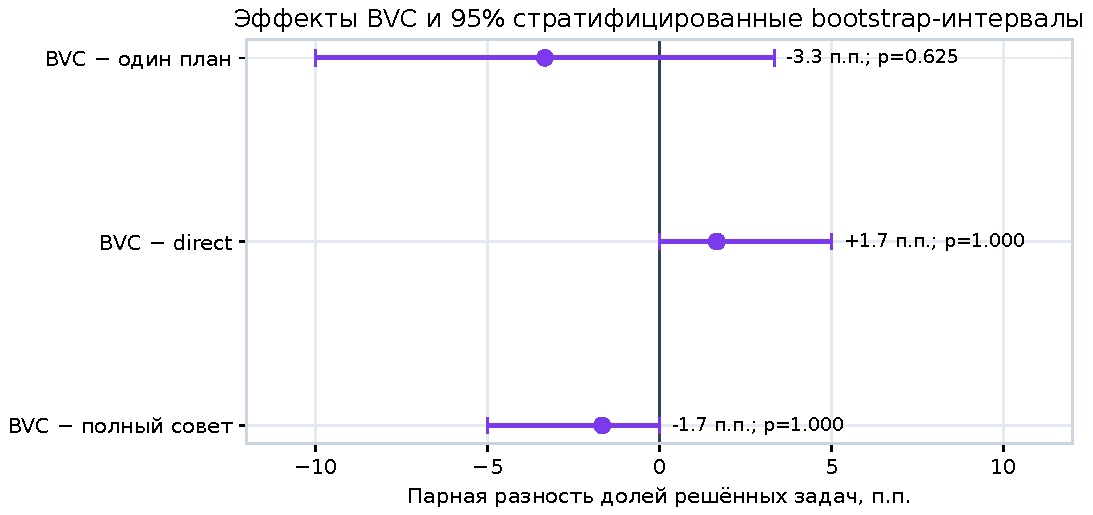
\includegraphics[width=0.9\textwidth]{fig_paired_effects}
\caption{Парные эффекты BVC относительно трёх заранее заданных baseline.}
\label{fig:paired}
\end{figure}

Полный совет решил 6/60, BVC --- 5/60; пять успехов совпали. Результаты
первичного contrast и полного совета не отменяют арифметику вторичного
сигнала против direct, но точно ограничивают его интерпретацию:
текущая выборка не подтверждает, что многоролевой upfront-анализ лучше
простого структурированного плана.

\begin{figure}[H]
\centering
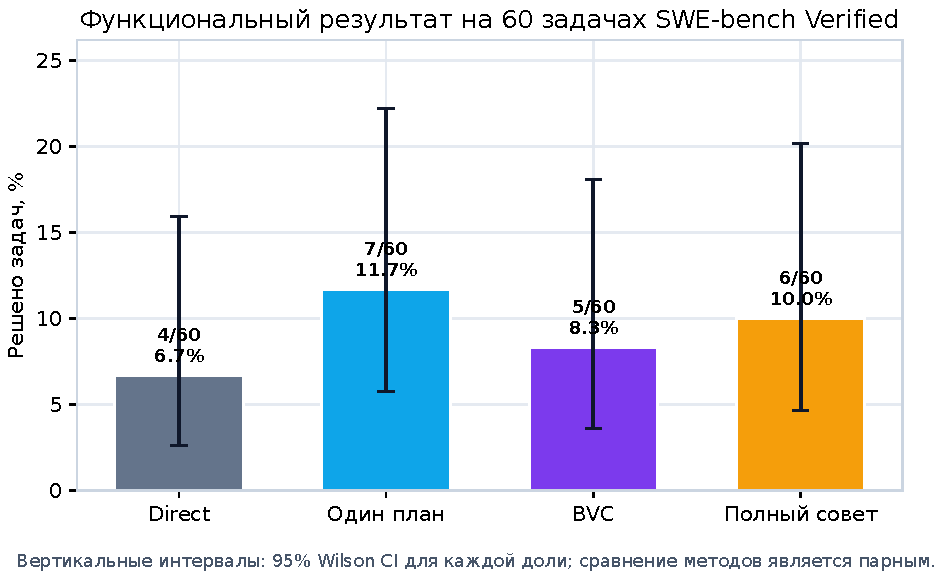
\includegraphics[width=0.9\textwidth]{fig_success_wilson}
\caption{Функциональные outcomes и 95\% Wilson-интервалы отдельных долей.}
\label{fig:rates}
\end{figure}

Wilson-интервал BVC равен \([3{,}6;18{,}1]\%\), direct ---
\([2{,}6;15{,}9]\%\) \cite{wilson1927}. Широкое перекрытие визуализирует
неопределённость, которую нельзя скрывать одной разностью \(+1{,}7\) \pp.

\section{Разговорная постановка и vibe coding}

\subsection{Функциональный результат}

\begin{table}[H]
\centering
\caption{Официальные outcomes на 15 задачах при смене стиля запроса.}
\label{tab:style}
\begin{tabular}{@{}lrrrr@{}}
\toprule
Метод & Формально & Разговорно & Разность & Согласие\\
\midrule
Direct & 0/15 & 2/15 & \(+13{,}3\) \pp & 13/15 (86,7\%)\\
Один план & 1/15 & 1/15 & \(0{,}0\) \pp & 15/15 (100,0\%)\\
BVC & 0/15 & 1/15 & \(+6{,}7\) \pp & 14/15 (93,3\%)\\
\bottomrule
\end{tabular}
\end{table}

\begin{figure}[H]
\centering
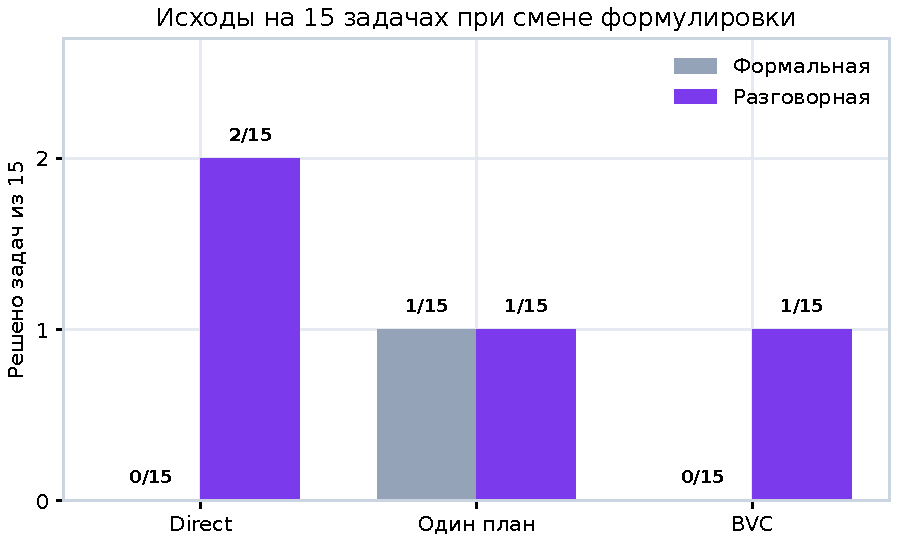
\includegraphics[width=0.88\textwidth]{fig_formal_vibe}
\caption{Формальная и разговорная формулировки при неизменном evaluator.}
\label{fig:vibe}
\end{figure}

В разговорной серии BVC и один план решили по одной задаче. Для BVC
формальный и разговорный outcome совпал на 14/15 instances. Наблюдаемое
изменение BVC равно \(+6{,}7\) \pp, но при одной дискордантной задаче
\(p=1{,}0\). Практически значим здесь не вывод о превосходстве языка, а
то, что разговорный ввод прошёл полный структурированный pipeline:
роли, gate, план, patch и официальные тесты.
Разности в таблице не превышают диапазон 0--2 успеха из 15, наблюдавшийся
между формальными повторами тех же методов; поэтому знак style-shift нельзя
интерпретировать причинно.

\subsection{Разность разностей}

Для сравнения относительного style-shift BVC и одного плана вычислена
разность разностей:
\[
\widehat{\delta}
=
(\widehat{p}_{B,\mathrm{vibe}}-\widehat{p}_{B,\mathrm{formal}})
-
(\widehat{p}_{S,\mathrm{vibe}}-\widehat{p}_{S,\mathrm{formal}})
=+6{,}7\ \text{\pp}.
\]
Стратифицированный bootstrap-интервал равен \([0{,}0;+20{,}0]\) \pp. При
малом \(n=15\) это только описательный post-hoc показатель: он не доказывает
причинный эффект стиля и задаёт гипотезу для серии с несколькими независимо
сгенерированными paraphrase.
Нулевая нижняя граница здесь также следует из конструкции: outcomes одного
плана совпали при обоих стилях, а у BVC нет задачи, решённой только в формальной
серии.

\section{Повторяемость при temperature = 0}

Для BVC числа решений по трём формальным запускам равны 0, 2 и 0 из 15.
Все три outcome совпали на 13/15 задачах; среднее попарное согласие
составило 91,1\%. Те же значения согласия получены для direct и одного
плана, хотя распределение успехов различалось.

\begin{figure}[H]
\centering
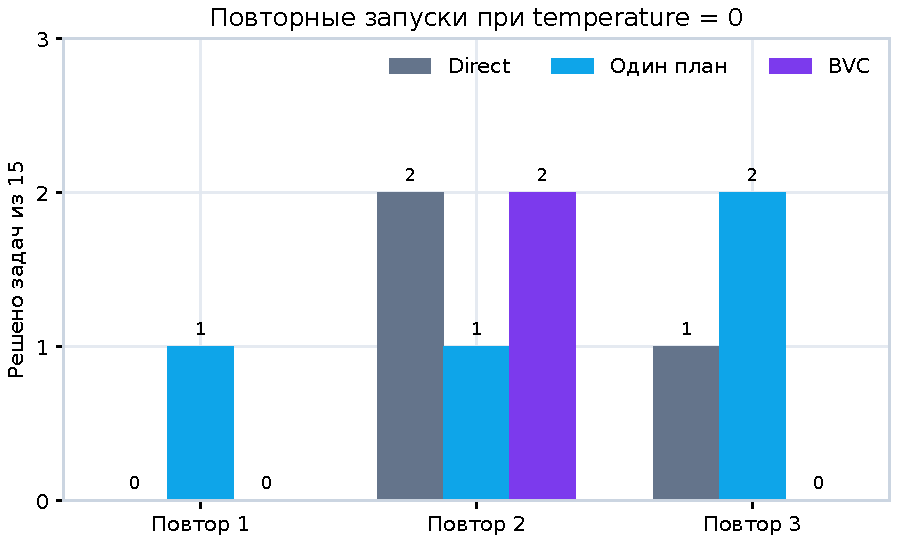
\includegraphics[width=0.88\textwidth]{fig_repeatability}
\caption{Вариация числа успешных patch между тремя повторами.}
\label{fig:repeat}
\end{figure}

Для продуктового интерфейса этот результат означает, что temperature \(=0\)
нельзя показывать как гарантию идентичного outcome. Попарное согласие 91,1\%
можно отображать только как наблюдаемую audit-метрику данной 15-задачной
серии, а не как калиброванную уверенность. Слой не оценивает дисперсию
60-задачного contrast напрямую, но колебание 0--2 успеха предупреждает, что
различие в одну--две задачи не является устойчивым доказательством качества.

\section{Адаптивный бюджет upfront-анализа}

Полный многоролевой маршрут требует 10 вызовов. BVC завершил
\BVCShort{}/60 задач после 6 вызовов и выполнил критику для
\BVCExtended{}/60. Среднее число вызовов:
\[
\overline{C}
=\frac{32\cdot6+28\cdot10}{60}
=7{,}8667.
\]
Относительно обязательного полного совета:
\[
1-\frac{7{,}8667}{10}=21{,}3\%.
\]

\begin{figure}[H]
\centering
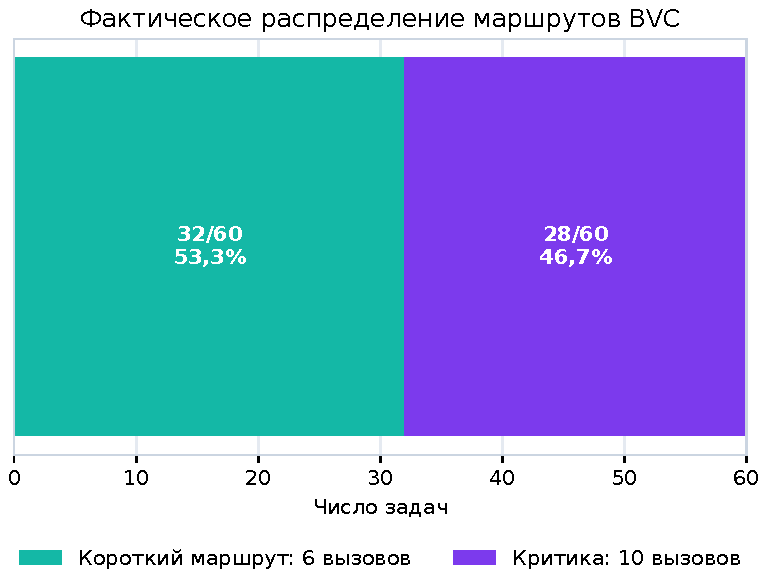
\includegraphics[width=0.82\textwidth]{fig_bvc_routes}
\caption{Маршрутизация BVC между стандартным и расширенным режимом.}
\label{fig:routes}
\end{figure}

\begin{table}[H]
\centering
\caption{Экономика BVC относительно полного совета.}
\label{tab:efficiency}
\begin{tabular}{@{}lrrr@{}}
\toprule
Метрика & Полный совет & BVC & Снижение\\
\midrule
Вызовы & \num{\FixedCalls} & \num{\BVCCalls} & \CallsSavedPct\%\\
Токены & \num{\FixedTokens} & \num{\BVCTokens} & \TokensSavedPct\%\\
Стоимость, руб. & \num{\FixedCost} & \num{\BVCCost} & \CostSavedPct\%\\
Стоимость на задачу, руб. & \num{\FixedCostTask} & \num{\BVCCostTask} &
\CostSavedPct\%\\
\bottomrule
\end{tabular}
\end{table}

Адаптивность особенно важна для vibe coding: человек может запросить
многоролевую проверку, не обязуясь оплачивать максимальный раунд на каждой
задаче. Диапазон 6--10 известен заранее, а фактический маршрут объясняется
числовыми диагностическими признаками.

\begin{figure}[H]
\centering
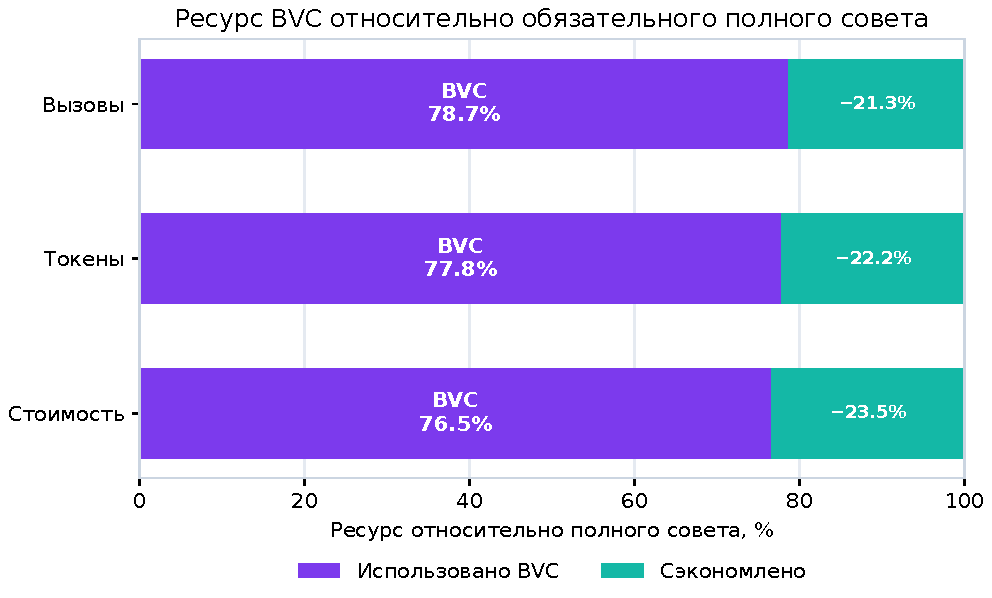
\includegraphics[width=0.9\textwidth]{fig_resource_normalized}
\caption{Фактический ресурс BVC как доля ресурса полного совета.}
\label{fig:resources}
\end{figure}

Агрегаты дополнительно проверены на уровне одинаковых задач. Для
\(\Delta X_i=X_{i,\mathrm{fixed}}-X_{i,\mathrm{BVC}}\) средняя парная
экономия равна \num{\CallsSavedTaskMean} вызова, \num{\TokensSavedTask}
токенов и \num{\CostSavedTask} руб. на задачу. Соответствующие 95\%
bootstrap-интервалы равны
\([\num{\CallsSavedTaskMeanLow};\num{\CallsSavedTaskMeanHigh}]\) вызова,
\([\num{\TokensSavedTaskMeanLow};\num{\TokensSavedTaskMeanHigh}]\) токенов
и \([\num{\CostSavedTaskMeanLow};\num{\CostSavedTaskMeanHigh}]\) руб.
Bootstrap выполнялся 10\,000 раз внутри medium/hard/very-hard страт;
положительное значение означает экономию BVC. При этом на уровне отдельных
задач BVC использовал больше токенов в 11/60 случаях и имел большую расчётную
стоимость в 10/60; агрегатная экономия не означает экономию на каждой задаче.

\begin{figure}[H]
\centering
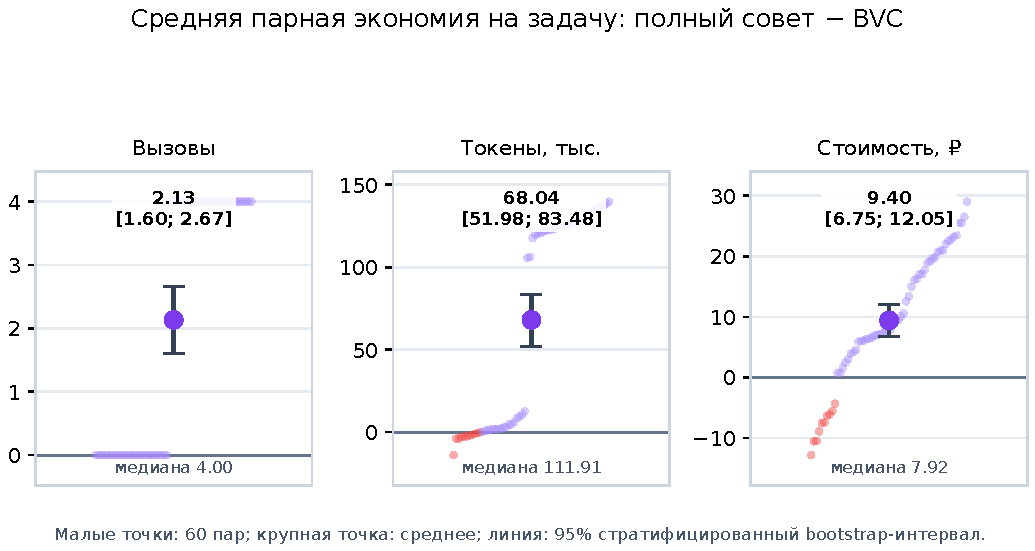
\includegraphics[width=0.9\textwidth]{fig_resource_paired_effects}
\caption{Парная экономия на задачу и 95\% стратифицированные
bootstrap-интервалы среднего.}
\label{fig:resource-paired}
\end{figure}

\section{Интеграция в Xynapse}

\subsection{Команда и момент подтверждения}

Дипломная архитектура \cite{khalilov2026} может использовать явную команду
\code{/bvc} или переключатель \enquote{Проверить план до изменения кода}.
До запуска интерфейс показывает верхнюю границу 10 вызовов; после первого
раунда --- выбранный маршрут. Отдельное подтверждение не требуется, если
пользователь уже включил режим и бюджет находится в заявленном диапазоне.

\subsection{Карточка плана}

Результат синтеза должен отображать:
\begin{itemize}
  \item root cause: файлы, символы и наблюдаемая причина;
  \item fix strategy: класс и шаги изменения;
  \item dependencies: контракты, которые необходимо обновить или сохранить;
  \item test coverage: существующие и новые проверки;
  \item \(D_{\mathrm{vote}}\), \(D_{\mathrm{cov}}\), причины gate;
  \item фактические вызовы, токены и оценочную цену.
\end{itemize}
Такая карточка является контрактом между предварительным анализом и
инструментальным агентом. Если агент отклоняется от списка файлов или
инвариантов, интерфейс может запросить новое решение, а не молча расширять
patch.

\subsection{Переход к инструментальному циклу}

После BVC начинается обычный цикл поиска, редактирования и тестирования:
\[
\text{план}\rightarrow
\text{правка}\rightarrow
\text{тесты}\rightarrow
\text{наблюдение}\rightarrow
\text{уточнение}.
\]
BVC не заменяет инструменты. Его проектная задача --- структурировать вход в
этот цикл: заранее предложить, что менять и как доказать корректность; данный
эксперимент не установил общего повышения качества. Результаты
официального evaluator в исследовании выполняют ту же роль наблюдения, которую
в IDE исполняют локальные тесты.

\subsection{Когда достаточно короткого режима}

Если роли независимо сходятся по локализации, стратегии и тестам, повторное
обсуждение не добавляется. Если обнаружена неполнота или существенное
расхождение, один раунд критики оплачивается автоматически. Наблюдаемая
выборка дала 53,3\% коротких маршрутов. Это конкретная основа для UI:
индикатор бюджета может показывать не абстрактную \enquote{сложность}, а
фактическую долю случаев, когда дополнительная критика понадобилась.

\section{Практические расчёты эффективности}

\subsection{Стоимость одного запуска}

Средняя расчётная стоимость BVC равна \num{\BVCCostTask} руб. на задачу.
Короткий маршрут в наблюдаемой выборке стоил в среднем
\num{\BVCShortCostMean} руб., расширенный --- \num{\BVCExtendedCostMean}
руб. Разность \num{16.84} руб. является описательным различием между группами
задач, выбранными gate. Она смешивает цену четырёх critique-вызовов с
различиями самих задач и поэтому не является причинной оценкой цены критики.

\subsection{Стоимость успешного результата}

BVC израсходовал \num{\BVCCost} руб. и решил пять задач:
\[
\frac{\num{\BVCCost}}{5}
=\num{\BVCCostResolved}\ \text{руб./решённую задачу}.
\]
Полный совет:
\[
\frac{\num{\FixedCost}}{6}
=\num{\FixedCostResolved}\ \text{руб./решённую задачу}.
\]
Описательная экономия BVC по этой нормировке равна 8,2\%. Из-за малого
знаменателя показатель не доказывает общего преимущества, но подтверждает,
что сокращение бюджета в данной серии не было куплено ростом наблюдаемой
цены успеха относительно полного совета.

\subsection{Цена дополнительной проверки}

Сравнение с direct отвечает на вопрос качества, но цена режимов структурно
различна: direct стоит в среднем \num{\DirectCostTask} руб., BVC ---
\num{\BVCCostTask} руб. Поэтому BVC следует включать не как постоянный
заменитель любой генерации, а как осознанную предварительную проверку в
задачах, где дополнительный анализ оправдан ценой ошибки. Эксперимент
показывает измеримый функциональный сигнал \(+1/60\), но не оценивает
стоимость производственного дефекта; такое решение остаётся за пользователем
или политикой IDE.

\section{Научная и практическая значимость}

Первый результат --- операционализирован пользовательский сценарий
\enquote{сначала обсудить, потом писать код}: момент включения, роли,
структура вывода и граница бюджета заданы явно.

Второй результат --- вторичный положительный task-paired сигнал относительно direct:
одна дополнительная решённая задача без потерь на общих успехах. Его сила
описана точно: \(+1{,}7\) \pp, \(p=1{,}0\), без заявления статистического
превосходства.

Третий результат --- BVC прошёл полный pipeline при одной разговорной
формулировке, дал 1/15 успех и 93,3\% согласия outcome со своей формальной
версией; это документирует сценарий, но не устанавливает общую устойчивость.

Четвёртый результат --- стоимость многоролевого анализа стала управляемой:
gate сократил токены на 22,2\% и расчётную стоимость на 23,5\% относительно
обязательной критики.

В совокупности эти данные поддерживают дальнейшее развитие Xynapse как IDE,
в которой пользователь может выбирать не только модель, но и проверяемый
режим принятия решения. Это и есть ключевая практическая польза алгоритма:
он встраивает между намерением пользователя и правкой кода ограниченный,
объяснимый этап проверки, глубина которого адаптируется по наблюдаемым
диагностическим признакам. Ссылка на диплом \cite{khalilov2026} фиксирует
происхождение архитектуры; числовая часть статьи основана на отдельном
исполняемом эксперименте.

\section{Границы интерпретации и следующий тест}

Основная выборка ограничена 60 задачами, а разговорная --- 15 задачами и
одним созданным моделью paraphrase на задачу. Здесь
\enquote{vibe coding} операционализирован только как однократная разговорная
переформулировка требования до генерации; интерактивное программирование с
последовательными уточнениями, инструментами и пользовательской обратной
связью не исследовалось. Не включён equal-budget best-of-\(k\) или
self-consistency baseline, поэтому работа не показывает, что многоролевая
декомпозиция является лучшим использованием того же бюджета. Контекст
ограничен BM25-выборкой, а patch создавался одним вызовом без тестовой обратной
связи. Число функциональных успехов мало, поэтому интервалы
широки. Следующий подтверждающий тест должен заранее зафиксировать новую
выборку, несколько независимых разговорных формулировок, primary-contrast
BVC--direct и достаточный объём для обнаружения эффекта порядка нескольких
процентных пунктов. Текущие данные подходят для постановки такой гипотезы,
но не для post-hoc заявления гарантированного улучшения. Кроме того,
актуальный аудит \dataset{} указывает на остаточные дефекты тестов и
контаминацию, из-за чего benchmark больше не рекомендуется как мера
frontier coding capability \cite{openai2026verifiedlimits}. Здесь он
используется как фиксированный одинаковый evaluator четырёх workflows, а не
как абсолютный рейтинг модели.

Три статьи проекта анализируют одну основную матрицу 240 запусков, а не три
независимые репликации: настоящая статья выделяет upfront-сценарий и
чувствительность к стилю, две другие --- адаптивный бюджет и аудируемость.

\section{Заключение}

Upfront BVC реализует конкретный и ценный пользовательский запрос: включить
многоролевую проверку до исправления ошибки или до передачи плана агентам.
В первичном сравнении он дал пять успешных patch против семи у одного плана;
преимущество и неухудшаемость не установлены. Во вторичном сравнении пять
успехов против четырёх у direct дают положительный описательный сигнал
\(+1{,}7\) \pp{} при adjusted-\(p=1{,}0\). В разговорной
серии BVC решил 1/15 и сохранил 93,3\% согласия с формальным outcome.
Адаптивный gate использовал короткий маршрут в 32/60 задачах и сократил
токены более чем на одну пятую относительно полного совета.

Практическая ценность BVC уже подтверждена там, где эксперимент имеет
достаточно прямое измерение: ресурсная адаптивность показана
напрямую, а улучшение качества пока является небольшим наблюдаемым сигналом,
не статистическим доказательством. Именно в такой форме результаты
экспериментально продолжают дипломный проект Xynapse
\cite{khalilov2026} и дают основу для следующей, заранее рассчитанной серии.
Алгоритм ценен не обещанием заменить инженерное суждение, а тем, что делает
предварительную проверку включаемой, ограниченной, объяснимой и измеримой.

\section*{Декларации}

Финансирование и конфликт интересов отсутствуют. LLM использовались для
генерации экспериментальных ответов, разговорных paraphrase и языковой
редакции; функциональный outcome определён официальным исполняемым evaluator,
а числовые значения вычислены из сохранённых JSON/JSONL. Диплом
\cite{khalilov2026} является источником архитектуры Xynapse/BVC, но не
источником экспериментальных результатов статьи.

\clearpage
\printbibliography[title={Литература}]
\end{document}
